\pagenumbering{arabic}

\chapter{Introduction}
\section{Problem}
Honeybees have a huge impact on the world around. Almonds in particular are completely dependent on honeybee pollination and because of this, sixty percent of the United States’ honeybees are sent to California. The honeybee population has been in a steady decline since the seventies. The population of honeybees has declined from 4 million to 2.5 million. This is partially due to a phenomenon called colony collapse disorder, which is when the majority of worker bees abandon a queen, food, young, and nurse bees. 

Colony collapse disorder is still largely unknown, and research has only just begun. Building a habitat monitoring system that can record data from a beehive and analyzing the data can help build a foundation of knowledge for studying this issue. This data would include audio from inside the hive, video above the entrance of the hive, as well as the temperature and humidity of the interior of the hive. The audio will help us listen to the health of the hive by listening for certain signals that the bees make occasionally, specifically piping and quacking. The video will be recording a top down view of the entrance of the beehive, which will allow monitoring of both bees leaving and returning to the hive everyday, in addition to predators or rivals attempting to enter the hive. Temperature and humidity are relevant for when the hive is dormant in the winter. If the air gets too humid, it can cause mold and if the air is too cold, which can cause a population decrease. 

\section{Goals}
Continuing on with this research, I would like to achieve two main goals. First, I would like to create a simple graphical user interface in which you could control the Raspberry Pi. This would allow inexperienced users to be able to control their systems. This user interface should allow a user to set all of their preferences, such as start times and stop times, as well as manually controlling the system. 
The next goal is to integrate a new system flow. Since many hives can be close in proximity to one another, it would be more efficient if you have a ‘middleman’ controller that all of the surrounding controllers would connect to for instruction. Figure 1.1 shows the updated data flow. 

\begin{figure}
    \centering
    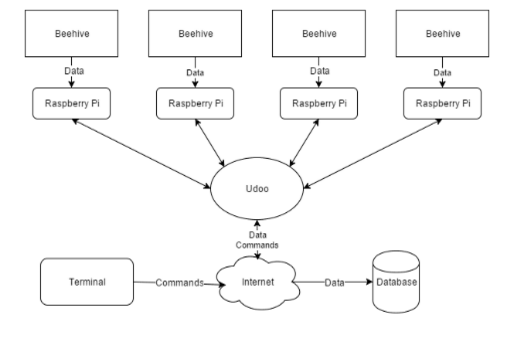
\includegraphics{udoo}
    \caption{Network with Raspberry Pis and a Udoo}
    \label{fig:my_label}
\end{figure}


In Figure 1.1, you can also see that you still connect via your terminal, but your commands are now routed through a Udoo. A Udoo is another microcontroller similar to the Raspberry Pi, but it comes with an advantage of being able to connect to a hard disk drive. This system would allow you many Raspberry Pis to connect to a single Udoo. This would simplify the process of connecting, since you would not need to connect to all four individually. Since the Udoo with be connected to all of the Raspberry Pis, it will also be a single location for all of their data. The data will then be uploaded in at one time during off peak hours.

\section{Motivation}

\section{Overview}

\chapter{Literature Review}
\section{Habitat and Animal Monitoring}
In the paper entitled “Analysis of animal monitoring technologies in Germany from an innovation system perspective”, they seek to analyse the full life cycle of animal monitoring technologies. Specifically, they study the development, generation, and use of animal monitoring technologies. However, this thesis focuses on the development of such systems. Based on expert interviews, workshops, and a Delphi survey, they were able to conclude a number of steps to ensure proper growth within the systems. These steps include: resource-based fostering of network management, high level of scientific education and research, and openness to new challenges and demands \cite{busse_analysis_2015}. 


A paper written by Lynch, Alderman, and Hobday studied the use of high resolution cameras to study the behavior of seabirds. The goal of the paper was to build a low cost and weather proof system that could reliably monitor the nesting habits seabirds. During their experiment, they used a camera system called Gigapan which allowed them to take a panoramic photograph of the entire area of the nesting grounds. This allowed them to get a much better view of the entire flock at once instead of using many individual cameras. Once the pictures were captured, they were sent to a server stored in their laboratory. It was concluded that the pictures taken could extend or enhance their data collection methods \cite{lynch_high-resolution_2015}.


Kumar and Hancke developed a system that could monitor both environmental and animal data. This data included body temperature, heart rate, air temperature, and humidity. They also claim to be able to read stress levels of individual animals corresponding to the thermal humidity index. They use a ZigBee and an attached microcontroller to relay the readings which are read through a GUI in real time. The sensors are placed around the neck of the animal inside a weatherproof container and the data is transmitted via ZigBee to a relay station. The relay station then interfaces directly with a PC where the GUI displays the data. They were able to show they were able to detect the health of the animals using this system \cite{kumar_zigbee-based_2015}. 


\section{Networking of Systems}
A study on wireless sensor networks took place on an island near Maine. During this study, they used a network of 43 nodes that would transmit data from the island to the internet. While the deployment time was relatively short, they were able to transmit over a million readings from the nodes. The paper argues that wireless sensor networks are a much more practical solution to habitat data collection. Some benefits that are listed are price, instant access to data as opposed to onsite data loggers, less habitat impact, and little to no need for human intervention. The paper concluded that nodes had a very high failure rate and failed to deliver any meaningful data for their research. It did show that when viewing sensor data, you could use the readings to predict when a node would fail \cite{polastre_analysis_2004}.


An analysis of two different subtypes of wireless sensor networks was done during a four month period. The two types of networks were single hop networks and multi hop networks. Single hop networks are nodes connected directly to a single source of internet, while a multi hop network would allow nodes to pass data between other nodes with the end goal being the router connected to the internet. During their experiment they used two different types of probes to record data: one recorded weather data and the other recorded data of birds inside burrows. Their conclusions of these networks were based on their battery life expectancy over the course of the experiment. The single hop network outperformed the life of the multi hop network. The majority of the weather nodes for the single hop network died around the 125 day mark while the multi hop nodes died around the 65 day mark. The burrowed nodes for both single hop and multi hop networks died around the 40 day mark. This was concluded to be an issue with a sensor drawing more power than expected \cite{szewczyk_analysis_2004}.


A paper written by YingMing and RenCheng focuses on the uses of wireless sensor networks and outlines a framework of use. While they found that most previous versions of wireless sensor networks used 8-bit MCUs at a low clock rate, they decided to use a 32-bit system that is compatible with a ZigBee. A ZigBee is a low power and inexpensive component that allows communication between other ZigBees within a certain radius. As their gateway node, they used two different systems. The first being a ZigBee to allow communication through the network to the sensors. The second was a General Packet Radio Service device that allowed data to be transmitted to a smartphone. They conclude that power consumption plays the biggest role within these networks and that everything within the system has to be optimized for power consumption \cite{yingming_novel_2008}.


Polastre proposes that wireless sensor networks are the future for scientific communities doing research on the environment. Since each sensor can be apart of the environment and have a very small impact it can prove to be much more advantageous than other more bulky equipment. Local storage of data allows these sensors to run aggregation, filtering, and compression algorithms. The ability for multiple sensors to communicate allows a group of nodes to perform more complex tasks, such as statistical sampling, data aggregation, and check system health. However, a full support system for these networks must be in place for the network to perform at full capacity. These include power management, sampling mechanisms, and a protocol for communication. Their system was deployed in two environments studying different  types of data. However, their system was able to handle the data acquisition and transmission \cite{polastre_design_2003}.
\chapter{Methodology}
\section{Introduction}
\section{Data Acquisition}
\subsection{Hardware}
\subsection{Software}
\subsection{Data Verification}
\section{Network Flow}
\subsection{Hardware}
\subsection{Single Hop Network}
\subsection{Network Health}
\section{Graphical User Interface}
\subsection{Requirements}
\subsection{Analysis}

\chapter{Results}
\section{Data Acquisition}
\section{Network Flow}
\section{Graphical User Interface}


\chapter{Conclusions and Future Work}
\section{Conclusions}
\section{Future Work}

\chapter{Timeline for Completion}
\begin{itemize}
\item July 22\textsuperscript{nd} to August 15\textsuperscript{th} -- Finish the first version of the GUI

\item August 16\textsuperscript{th} to August 31\textsuperscript{st} -- Implement wireless sensor network

\item September 1\textsuperscript{st} to September 15\textsuperscript{th} -- Analyse network health and performance

\item September 16\textsuperscript{th} to September 30\textsuperscript{th} -- Implement data verification system

\item October 1\textsuperscript{st} to October 31\textsuperscript{st} -- Implement analysis software within GUI

\item November 1\textsuperscript{st} to November 13\textsuperscript{th} -- Analyse accuracy of all data readings and network health

\item November 14\textsuperscript{th} to November 28\textsuperscript{th} -- Edit prospectus, if needed

\item November 28\textsuperscript{th} -- Submit prospectus

\item December 15\textsuperscript{th} to January 15\textsuperscript{th} -- Write first draft of methodology

\item January 15\textsuperscript{th} to January 22\textsuperscript{nd} -- Get it revised

\item January 22\textsuperscript{nd} to February 10\textsuperscript{th} -- Write first draft of results

\item February 10\textsuperscript{th} to February 17\textsuperscript{th} -- Get it revised

\item February 17\textsuperscript{th} to March 17\textsuperscript{th} -- Write first draft of conclusion, future work, and any other parts

\item March 17\textsuperscript{th} to April 1\textsuperscript{st} -- Get it revised, and proof-read the whole thing

\item April 5\textsuperscript{th} -- Announce defense

\item April 10\textsuperscript{th} -- Double check formatting

\item April 14\textsuperscript{th} to April 23\textsuperscript{rd} -- Defend and make corrections

\item April 24\textsuperscript{th} -- Turn in to grad school
\end{itemize}